
\chapter{FEST-Swing}\label{chap:fest-swing}

FEST (Fixtures for Easy Software Testing) is a collection of libraries whose mission is to simplify software testing. It is composed of various modules, which can be used with TestNG or JUnit. The most significant module is the FEST-Swing module.

The Swing module provides a simple and intuitive API for functional testing of Swing user interfaces, resulting in tests that are compact, easy to write, and read like a specification. Tests written using FEST-Swing are also robust. FEST simulates actual user gestures at the operating system level, ensuring that the application will behave correctly in front of the user. It also provides a reliable mechanism for GUI component lookup that ensures that changes in the GUI's layout or look-and-feel will not break the tests \cite{FESTMain}.

\section{Introduction}\label{sec:intro}

A FEST-Swing test is testing either individual frames (the building blocks of a UI), or entire Swing applications or Applets. FEST simulates actual user gestures (mouse movements, keys presses) at the operating system level, ensuring that during the application will behave in the same way as in the front of the user. It uses AWT Robot, which generates events in the platform's native input queue. Thus, the test needs to create the components and make them visible on the screen, and the tests will actually moves the mouse cursor, and not just only generates mouse move events.

\section{Architecture}\label{sec:architecture}

FEST Swing's component fixture architecture is separated into several layers (from bottom to top):
\begin{enumerate}
\item BasicRobot: Simulates a user interacting with a mouse and keyboard. It uses the AWT Robot to generate native input events.
\item Component driver: This layer does all the ``heavy lifting.'' All interaction with a GUI component is done in this layer. It knows how to simulate events and check the state of a specific GUI component. For example, JComboBoxDriver knows how to simulate a user using a JComboBox (selecting a particular element) and how to verify the state of it (which element should be selected.)
\item Component fixture: This layer sits on top of the driver. It provides a fluent interface to that and makes the API easier to write and read. Users of FEST write their GUI tests using fixtures, not drivers. There is one fixture per Swing component, and each fixture has the same name as the Swing component they can handle ending with ``Fixture.'' For example, a JButtonFixture knows how to simulate user interaction and verify state of a JButton. Fixtures can be considered the ``user interface'' of the FEST-Swing library.
\end{enumerate}

The architecture also supports extensions, so developers of application using custom Swing components can write their own fixtures and component drivers.

\section{Example}\label{sec:example}

Writers of GUI tests need to use the fixtures located in the package org.fest.swing.fixture. These fixtures provide specific methods to simulate user interaction with a GUI component and they provide assertion methods that verify the state of the GUI component. Although it is possible to work with the FEST BasicRobot directly, the BasicRobot is too low-level and requires considerably more code than the fixtures.

As a concrete example, let us consider a very simple JFrame that contains a JTextField, a JLabel and a JButton, and component has its unique name. The expected behavior of this GUI is the following: when user clicks on the JButton, the text of the JTextField should be copied to the JLabel. (Figure \ref{fig:example_jframe}) 

\begin{figure}[h!] \label{fig:example_jframe}  
  \centering
    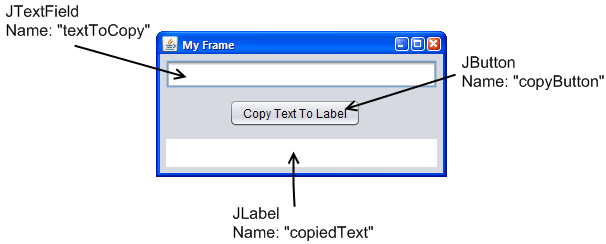
\includegraphics[width=0.6\textwidth]{images/example_jframe.png}
  \caption{A very simple JFrame that contains a JTextField, a JLabel and a JButton.}
\end{figure}

To the frame, the test's setup method needs to create the frame (in the EDT, delegating it with GuiActionRunner), create a fixture for it, and make it visible (Figure \ref{fig:example_setup_method}).

\begin{figure}[h!] \label{fig:example_setup_method}
\begin{lstlisting}
protected void onSetUp() {
    MyFrame frame = GuiActionRunner.execute(new GuiQuery<MyFrame>() {
        protected MyFrame executeInEDT() {
            return new MyFrame();  
        }
    });
    window = new FrameFixture(robot(), frame);
    window.show(); // shows the frame to test
}
\end{lstlisting}
\caption{The setup method creating the frame and the fixture, and making it visible.}
\end{figure}

The test method can use the fixture to simulate a user interacting with a GUI in order to verify that such GUI behaves as we expect. The user interactions and the assertions in the test are fluent and simple. The method looks up the UI components by their unique names. (Figure \ref{fig:example_test_method})

\begin{figure}[h!] \label{fig:example_test_method}
\begin{lstlisting}
@Test 
public void shouldCopyTextInLabelWhenClickingButton() {
    window.textBox("textToCopy").enterText("Some random text");
    window.button("copyButton").click();
    window.label("copiedText").requireText("Some random text");
}
\end{lstlisting}
\caption{The test method.}
\end{figure}

It is important to mention that besides testing individual components that build up an application, FEST-Swing also supports testing entire applications. In such cases, the first tests starts up the application with ApplicationLauncher that understands how to launch an application using its main method. Once the application is started, the test just needs to find the application's main window.

\section{Threading model}\label{sec:threading_model}

The documentation of FEST-Swing strongly advises to respect Swing's threading rules \cite{OracleSwingThreading} both in the tests and in the tested application (this remains only an advice because Swing itself does not enforce thread safety). In short, the cardinal rule is the following: creation and access (both read and write) of Swing components should be done in the Event Dispatch Thread (EDT.) Since JUnit and TestNG tests do not run on the EDT, creation and any direct access in the tests to Swing components should be delegated to EDT via the utility class GuiActionRunner (or via other tools).

To ensure that the threading rules are respected throughout the tests and the tested application, FEST Swing provides the class FailOnThreadViolationRepaintManager. It forces a test failure if access to Swing components is not performed on the EDT. However, it only detects component creation and writing, and is unable to detect read operations (component creation and writing triggers repaint events, but read does not).

\section{Limitations}\label{sec:limitations}

Because FEST-Swing is actually simulating user interaction, it needs an environment very similar to actual user environments: the tested application needs to be active and in focus, and needs to move the mouse. Therefore, that machine that the tests run on cannot be used for the entire duration of the tests. In addition, the tests probably fail whenever another applications unexpectedly gets the focus and covers the application's window (the mouse no longer clicks the correct application). This can become a burden because UI tests, by their nature, can take a significant amount of time to execute and especially when using agile development methods, it is preferable to run them frequently.

Because of this, it is common to delegate the tests to Continuous Integration (CI) systems (e.g. Hudson/Jenkins, TeamCity etc.) When the CI platform is based Linux, BSD or UNIX-style operating systems, it is common that the server does not even have the X Window system, running applications with UI impossible. For this case, Xvfb offers a simple and straightforward solution \cite{FESTxvfb}.

However, if the target platform is Windows, there are a whole set of issues, and the known solutions are problematic, and are very complicated and time consuming to setup. \cite{HudsonUnderWindows} \cite{Cacio_Tta_FEST}

To overcome all of these limitations, OpenJDK’s project Caciocavallo can be used \cite{Cacio_Tta_FEST} to provide a graphics stack for the Java VM that is completely independent from the environment, eliminating any need for platform-dependent setup for CI systems. It renders everything into a virtual screen (which is simply a BufferedImage object), and is driven solely by AWT Robot events. However, this also has its own limitations; the most important being that drag-and-drop \cite{IntroDnD} is unsupported, thus it needs certain workarounds (see \fullref{chap:simulated-dnd}).

\chapter{User Action and Adapter design pattern}\label{chap:user-actions-adapters}

The users using an application with a UI typically interact with it by executing a series of operations that change the application's state. These operations might themselves be consisting of multiple operations of the UI components, changing the UI's state and, indirectly, changing the application's internal state. UI test simulating the users can incorporate in their architecture the concept of separation: the tests can interact with a user action layer (consisting of the actions the user can do with the application), and the user actions can interact with an adapter layer that itself interacts with the UI components (e.g. by using FEST-Swing).

The same separation applies to the tests’ assertions: the tests assert the application's state through the user actions, and the user actions assert the UI's state, and thus, indirectly, assert the application's internal state.

\section{Adapters}\label{sec:adapters}

The adapters understand how to execute operations on the application by using the UI components. 

For example, to create a new text file in an editor application supporting multiple types of files, the user typically needs to click on the File menu, then on the menu item New, and then on the sub-menu-item Text file. The combinations are usually limited (the submenu-item cannot be clicked without clicking the menu item first), and sometimes require some checking (if the File menu is already visible for whatever reason, the test should not click it again because that would only close the menu).

These operations come from the functional specification of the application, and their implementation details are only dependent on the UI design. These operations can be structured into adapters, where each logically bound component group can have a corresponding Adapter class (e.g. FileMenuAdapter), where the methods are the operations (e.g. FileMenuAdapter\#clickNewTextFile()). The adapter class can have a fixture for each Swing component, and the methods can directly interact with them.

This approach also leads to tests that are more resistant to UI changes, requiring less code change for each UI design change. For example, if the in the UI design of the above text editor the Text file menu item is moved directly into the File menu under the name New text file, only the appropriate adapter class needs to be modified, while all the tests using this operation are left unchanged. Whereas, if the code using the fixtures and clicking on the menu items was present in all the tests, such a change would need all the tests to be changed.

\section {User actions}\label{sec:user-actions}

The user actions understand how to execute operations of the application by using the adapters. 

For example, let us consider a case where the user wants to save the file in the current editor of an editor application with a new name. The user needs to click the Save as menu item, resulting in the appearance of a browser dialog. After that, he needs to enter the new file name into a text box, and then needs to click the OK button of the dialog, and finally wait for the dialog to disappear. In this case, the file menu can have an adapter; the file browser dialog can have an adapter; and using both of them in the same time in a given way can represent a user action. For example, the user actions related to the current edited document can be grouped into a user action class (EditorUserAction), and where the methods are the user actions (EditorUserAction.saveAs(newFileName)).

